% Multiple Sequence Alignment
%
% Simple examples of multiple sequence alignment

\subsection{Multiple Sequence Alignment}

\begin{frame}
\frametitle{Quick Outline of MSA}
\begin{itemize}
  \item More difficult than pairwise alignment - no quick algorithm for optimal alignment
  \item Many methods progressive:
  \begin{enumerate}
    \item Build rough tree
    \item Conduct pairwise alignments from leaves to root
  \end{enumerate}
  \item Tree-based progressive methods highly dependent on initial tree$\ldots$
  \item Alignments can be compared directly (M-COFFEE)
\end{itemize}
\end{frame}

\begin{frame}
\frametitle{Example protein set MSA}
The example file \texttt{glucanase.fasta} contains:
\begin{itemize}
\item Reference protein \texttt{YP\_052458.1}, an endo-1,4-D-glucanase
\item Its RBBH from the prodigal gene predictions on \texttt{chrA.fasta}
\item Its RBBH from the prodigal gene predictions on \texttt{chrB.fasta}
\item Its RBBH from the prodigal gene predictions on \texttt{chrC.fasta}
\item Its RBBH from the prodigal gene predictions on \texttt{chrD.fasta}
\end{itemize}
If these are all orthologues, they should align nicely.
\end{frame}

\begin{frame}[fragile]
\frametitle{Clustal Omega MSA example}
Using example FASTA file of sequences:
\begin{lstlisting}[language=bash]
$ clustalo -i glucanase.fasta -o glucanase_clustalo.aln --outfmt=clustal
\end{lstlisting}
\end{frame}

\begin{frame}[fragile]
\frametitle{T-COFFEE MSA example}
Using same FASTA file of sequences:
%note that M-COFFEE performs consensus MSA using several methods
%but will they all be installed?
\begin{lstlisting}[language=bash]
$ t_coffee -infile glucanase.fasta -outfile glucanase_tcoffee.aln
\end{lstlisting}
\end{frame}

\begin{frame}[fragile]
\frametitle{JalView example}
Visualisation of the two MSAs generated above with JalView:
\begin{lstlisting}[language=bash]
$ Jalview &
\end{lstlisting}
\begin{itemize}
\item Menu ``File'', ``Input Alignment'', ``from File''.
\item Select ``Clustal (.aln)'' for the file type
\item Select your generated alignment file.
\end{itemize}
\end{frame}

\begin{frame}[fragile]
\frametitle{Clustal Omega \& T-COFFEE alignments in JalView}
\begin{center}
%TODO - Crop
Clustal Omega: \\
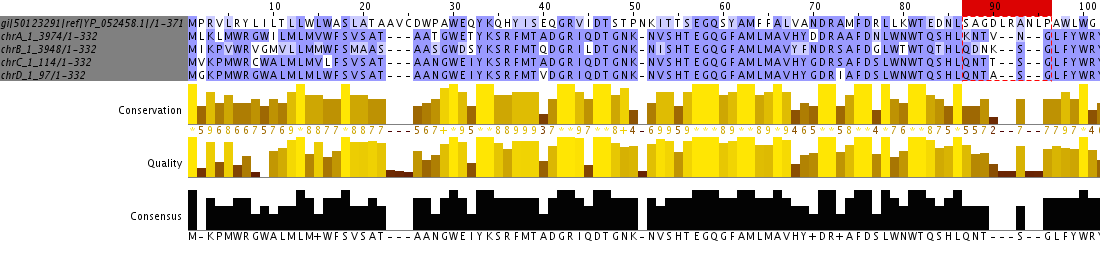
\includegraphics[width=\textwidth]{images/glucanase_clustalo.png} \\
T-COFFEE: \\
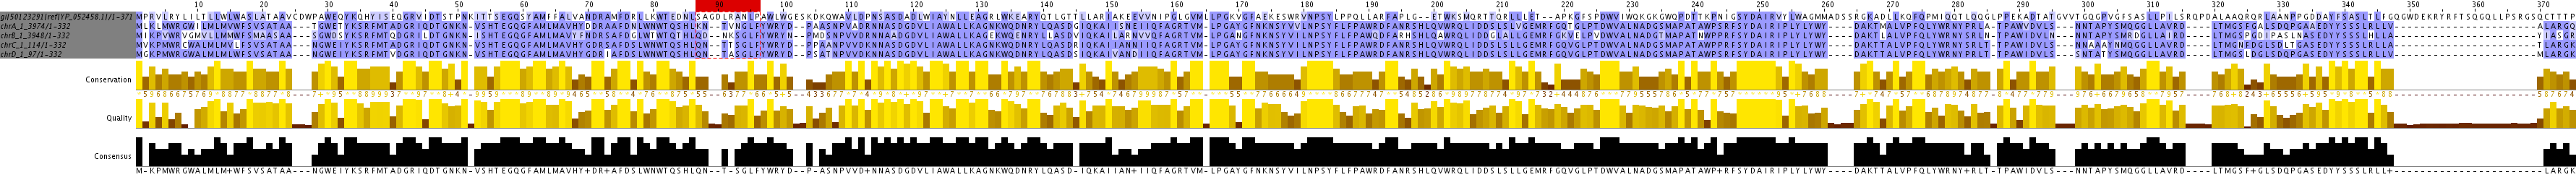
\includegraphics[width=\textwidth]{images/glucanase_tcoffee.png}
\end{center}
\end{frame}

\begin{frame}[fragile]
\frametitle{Clustal Omega \& T-COFFEE alignments in JalView}
\begin{center}
\begin{itemize}
\item Clustal Omega \& T-COFFEE gave different alignments
    \begin{itemize}
    \item e.g. region in red, and many more cropped on right
    \end{itemize}
\item The residues are coloured using the BLOSUM62 score
\item The proteins from draft chromosomes A, B, C and D are...
    \begin{itemize}
    \item Very similar to each other
    \item Only $30$ -- $35\%$ identical to the reference protein
    \item Probably \textit{not} orthologues of the reference protein
    \item Include minimum identity and coverage thresholds for RBBH!
    \end{itemize}
\end{itemize}
\end{center}
\end{frame}